
\begin{figure}
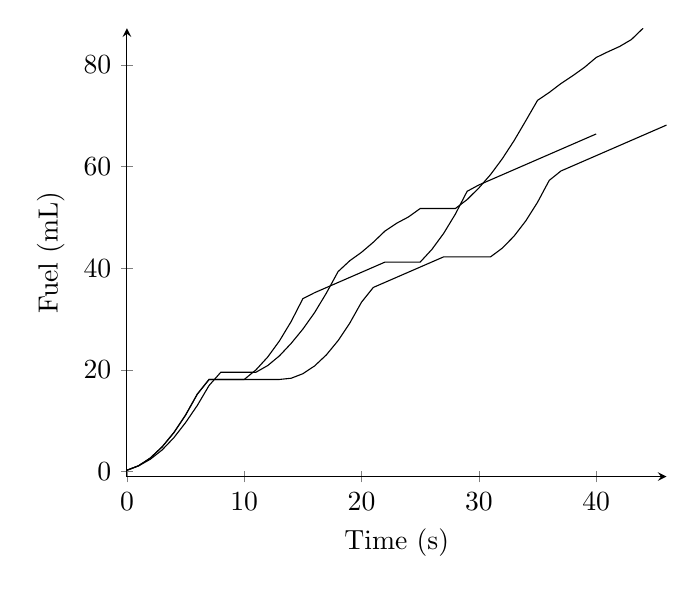
\begin{tikzpicture}
\begin{axis}[
legend style={
	anchor=west
},
axis x line=bottom,
axis y line=left,
ymin=-1,
point meta=explicit symbolic,
xlabel=Time (s),
ylabel=Fuel (mL)
]
\addplot[] coordinates {
(0, 0.239885513361)
(1, 1.13183007041)
(2, 2.66515136892)
(3, 4.83562037156)
(4, 7.64546130585)
(5, 11.1033516642)
(6, 15.2244222039)
(7, 18.1101790691)
(8, 18.1101790691)
(9, 18.1101790691)
(10, 18.1101790691)
(11, 18.1101790691)
(12, 18.1101790691)
(13, 18.1101790691)
(14, 18.3500645825)
(15, 19.2420091395)
(16, 20.775330438)
(17, 22.9457994406)
(18, 25.7556403749)
(19, 29.2135307333)
(20, 33.334601273)
(21, 36.2203581382)
(22, 37.2243480012)
(23, 38.2283378642)
(24, 39.2323277273)
(25, 40.2363175903)
(26, 41.2403074533)
(27, 42.2442973163)
(28, 42.2442973163)
(29, 42.2442973163)
(30, 42.2442973163)
(31, 42.2442973163)
(32, 43.9663713234)
(33, 46.325579037)
(34, 49.3260549204)
(35, 52.9783867013)
(36, 57.2996153725)
(37, 59.1482030816)
(38, 60.1521929446)
(39, 61.1561828076)
(40, 62.1601726706)
(41, 63.1641625337)
(42, 64.1681523967)
(43, 65.1721422597)
(44, 66.1761321227)
(45, 67.1801219858)
(46, 68.1841118488)
};
\addplot[] coordinates {
(0, 0.239885513361)
(1, 1.13183007041)
(2, 2.66515136892)
(3, 4.83562037156)
(4, 7.64546130585)
(5, 11.1033516642)
(6, 15.2244222039)
(7, 18.1101790691)
(8, 18.1101790691)
(9, 18.1101790691)
(10, 18.1101790691)
(11, 19.9984939445)
(12, 22.5243992186)
(13, 25.6937135242)
(14, 29.518708759)
(15, 34.0181100857)
(16, 35.1911290535)
(17, 36.1951189166)
(18, 37.1991087796)
(19, 38.2030986426)
(20, 39.2070885056)
(21, 40.2110783687)
(22, 41.2150682317)
(23, 41.2150682317)
(24, 41.2150682317)
(25, 41.2150682317)
(26, 43.7196666993)
(27, 46.867376332)
(28, 50.6702539604)
(29, 55.14680968)
(30, 56.3938811237)
(31, 57.3978709868)
(32, 58.4018608498)
(33, 59.4058507128)
(34, 60.4098405758)
(35, 61.4138304389)
(36, 62.4178203019)
(37, 63.4218101649)
(38, 64.4258000279)
(39, 65.4297898909)
(40, 66.433779754)
};
\addplot[] coordinates {
(0, 0.239885513361)
(1, 1.10670878636)
(2, 2.41451104245)
(3, 4.23417191665)
(4, 6.64678345996)
(5, 9.61829859551)
(6, 12.9982235193)
(7, 16.9136988622)
(8, 19.5298934224)
(9, 19.5298934224)
(10, 19.5298934224)
(11, 19.5298934224)
(12, 20.8453667372)
(13, 22.7580511721)
(14, 25.2106613699)
(15, 28.027471394)
(16, 31.2775371538)
(17, 35.1057845861)
(18, 39.3421975106)
(19, 41.4862175556)
(20, 43.1434336428)
(21, 45.1161151877)
(22, 47.3278691768)
(23, 48.8715249532)
(24, 50.0990342603)
(25, 51.7576835682)
(26, 51.7576835682)
(27, 51.7576835682)
(28, 51.7576835682)
(29, 53.5167023999)
(30, 55.8023161832)
(31, 58.4465475943)
(32, 61.564391381)
(33, 65.1066944773)
(34, 69.0360773549)
(35, 73.0391455021)
(36, 74.6042066214)
(37, 76.361051147)
(38, 77.8915307178)
(39, 79.5361615208)
(40, 81.4834975643)
(41, 82.6047456226)
(42, 83.6547636369)
(43, 85.0120671015)
(44, 87.2455209343)
};

\end{axis}
\end{tikzpicture}
\label{tik:50:14_V, 15_N, 17_S, 17_S.-60, 20_O, 21_O}
\caption{50 percent diving with GSC on route $14_V, 15_N, 17_S, 17_S.-60, 20_O, 21_O$}
\end{figure}
